\documentclass[a4paper,10pt,parskip]{scrartcl}
\usepackage[utf8]{inputenc}
\usepackage[ngerman]{babel}
\usepackage[T1]{fontenc}
\usepackage{lmodern}
\usepackage{amsmath}
\usepackage{amsfonts}
\usepackage{amssymb}
\usepackage{amsthm}
\usepackage{siunitx}
\usepackage{epsfig}
\usepackage{tikz}
\usepackage[lined,algoruled,linesnumbered]{algorithm2e}
%% \usepackage{algpseudocode}
%% \usepackage{algorithm}
\usepackage{graphicx}
\usepackage{placeins}

% an seitenbreite angepasste tabellen
\usepackage{booktabs}
\usepackage{tabularx} % page-width
\usepackage{adjustbox}

% coole inline-todos :)
\usepackage[colorinlistoftodos,prependcaption]{todonotes}

\renewcommand{\arraystretch}{1.5}

\usetikzlibrary{shapes.geometric, positioning, calc, shapes, fit, backgrounds}

\title{Projektausarbeitung \\\vspace{.5cm} \large gt Scaffolder: Eine Scaffolding-Software}

\author{Dorle Osterode, Lukas Götz \& Stefan Dang}
\date{}

\begin{document}
\maketitle{}
\thispagestyle{empty}
\begin{abstract}
  \todo{wollen wir ein abstract haben?}
\end{abstract}

\newpage{}
\setcounter{page}{1}
\section{Einleitung}
\todo{was ist DAS scaffolding Problem?}

Nach der Assemblierung von Sequenzen ist das Zielgenom oftmals noch
nicht vollständig rekonstruiert. Die rekonstruierten Sequenzabschnitte
(Contigs) sind dabei unabhängig voneinander und die relative Anordnung
sowie die Orientierung sind unbekannt. Diese Lücken (Gaps) in der
Zielsequenz entstehen oft durch ungleichmäßige Abdeckung durch die
Sequenzierung sowie repetitive Teilsequenzen. Durch repetitive
Teilsequenzen können die Contigs nicht in eine eindeutige Reihenfolge
gebracht werden.

Durch das Scaffolding nach der Assemblierung sollen die Contigs
relativ zueinander angeordnet werden, sodass zusätzlich auch die
Orientierung stimmt. Um dieses Verfahren anwenden zu können müssen
Distanzinformationen zwischen den Contigs vorhanden sein. Diese
Informationen stammen normalerweise aus \textit{paired-end}- oder
\textit{mate-pair}-Sequenzierung.

Beim Scaffolding wird ein Graph zur Repräsentation der Beziehungen
zwischen den Contigs verwendet. Dieser Graph enthält für jeden Contig
einen Knoten und es gibt Kanten zwischen zwei Knoten, wenn es ein
Read-Paar gibt, dass die durch die Knoten repräsentierten Contigs
verbindet. Die Kanten enthält dabei Informationen über die Distanz und
die Orientierung.

Nach Huson (2002) \cite{Huson:2002kf} ist das Scaffolding Problem
NP-vollständig. Dabei ist das Scaffolding die Ermittlung des optimalen
Pfades (Pfad mit maximalem Kantengewicht) jeder
Zusammenhangskomponente des Scaffolding-Graphen. Um diese Komplexität
zu umgehen werden Heuristiken zur Bestimmung eines guten Pfades für
jede Zusammenhangskomponente verwendet.

\section{Ziel des Projektes und Arbeitsvorgehen}
\subsection{Ziel des Projektes}
Ziel des Projektes war die Implementierung und Evaluierung einer
Scaffolding-Software. Dabei sollten die in der GenomeTools-Bibliothek
\cite{Gremme:2013} vorhandenen Konzepte und Infrastruktur verwendet
werden. Zusätzlich sollte die Scaffolding-Software mit den Ausgaben
des Assemblers ReadJoiner kompatibel sein.

Um diese Ziele zu erreichen wurde der Scaffolder aus der SGA-Pipeline
\cite{Simpson:2012ef} als Vorlage verwendet. Dieses Programm wurde
ausgewählt, da es sehr gute Ergebnisse erzielt \cite{Hunt:2014dh}. Da
die SGA-Pipeline allerdings viele Abhängigkeiten hat und deshalb nicht
einfach zu installieren ist und zusätzlich die Methodik des
Scaffoldings nicht hinreichend dokumentiert ist, sollte die Methodik
aufgeklärt und der Scaffolding-Algorithmus reimplementiert werden.

\subsection{Arbeitsvorgehen}
Zuerst wurden die verwendeten Datenformate und die Algorithmen
aufgeklärt. Da diese nicht hinreichend dokumentiert waren, mussten
diese Informationen aus dem Source-Code extrahiert werden.

Die so erhaltene Vorlage wurde leicht modifiziert, um sowohl Laufzeit
als auch Speicherplatz einzusparen. Unklarheiten in der Methodik wurden
dabei weitestgehend erst übernommen, um die Ergebnisse reproduzieren
zu können.

Diese Algorithmen wurden in der Programmiersprache C
implementiert. Dabei wurde gt Scaffolder zuerst so designet, dass es
die gleichen Eingabedateien erforderte wie SGA-Scaffold und die
gleichen Ausgaben produzierte, damit die Ergebnisse verglichen werden
konnten.

Um die Implementation zu testen wurden verschiedene Testdaten
ausgesucht. (\todo{hier mehr dazu schreiben!!!})

Anhand der Testdaten wurde gt Scaffolder evaluiert.

\section{Methoden}
\subsection{Übersicht der Schritte}

\begin{figure}
    \begin{tikzpicture}[every node/.style={font=\footnotesize}]
    \node[] (input1) {Contigs};
    \node[left of=input1, xshift=-1cm] (eingabe) {\textbf{Eingabe:}};
    \node[below of=eingabe, yshift=-5cm] (ausgabe) {\textbf{Ausgabe:}};
    \node[right of=input1, align=center, xshift=2cm] (input2) {Distanz-\\informationen};
    \node[right of=input2, xshift=2cm] (input3) {A-Statistik};

    \node[below of=input1, yshift=-.5cm, anchor=west] (titel) {gt Scaffolder};
    \node[rectangle, draw, anchor=west, below of=titel, xshift=1cm, rounded corners, fill=black!10, yshift=.25cm] (konstruktion) {Konstruktion des Graphen};
    \node[rectangle, draw, anchor=west, below of=konstruktion, xshift=.95cm, rounded corners, fill=black!10, yshift=.25cm] (selektion) {Selektion relevanter Knoten und Kanten};
    \node[rectangle, draw, anchor=west, below of=selektion, xshift=.80cm, rounded corners, fill=black!10, yshift=.25cm] (ermittlung) {Ermittlung aller Zusammenhangskomponenten (ZK)};
    \node[rectangle, draw, anchor=west, below of=ermittlung, xshift=-.65cm, rounded corners, fill=black!10, yshift=.25cm] (pfade) {Bestimmung des besten Pfades für jede ZK};

    \begin{pgfonlayer}{background}
    \node[draw, fit={(titel) (konstruktion) (selektion) (ermittlung) (pfade)}, rounded corners, fill=black!20] (back) {};
    \end{pgfonlayer}

    \node[below of=back, yshift=-2cm, xshift=-1.5cm] (output1) {Scaffolds};
    \node[right of=output1, align=center, xshift=2cm, yshift=-.25cm] (output2) {(rekonstruierte\\Sequenzen)};
    \node[above of=output1] (dummy) {};

    \path[->, thick]
    (input1) edge (back)
    (input2) edge (back)
    (input3) edge (back)
    (back) edge (output1)
    (back) edge (output2);
  \end{tikzpicture}
    \caption{\label{abb: gtscaffolder}Schematische Darstellung des Programmablaufs von gt Scaffolder.}
\end{figure}

In Abbildung \ref{abb: gtscaffolder} ist der Programmablauf von gt
Scaffolder schematisch dargestellt. (\todo{kurz beschreiben!!!})

\subsection{Eingabe}
Als Eingabe werden die Contigs im FASTA-Format, die
Distanzinformationen aus der \textit{paired-end}-
bzw. \textit{mate-pair}-Sequenzierung und die Astatistik der einzelnen
Contigs benötigt. gt Scaffolder benötigt dabei die
Distanzinformationen bezogen auf die Contigs, d.h. die Read-Paare
müssen zurück auf die Contigs gemappt und daraus die Distanz- sowie
Orientierungsinformation für die Contigs berechnet worden sein. Die
Astatistik ist ein statistisches Maß dafür, wie repetitiv eine Sequenz
ist \cite{Myers:2005iq}.

\subsection{Graphkonstruktion}
Aus den Contigs und den Distanzinformationen wird der
Scaffolding-Graph konstruiert. Dabei wird für jeden Contig, der eine
Mindestlänge von 200 bp überschreitet und eine Astatistik größer 19
hat, ein Knoten in den Graph eingefügt. Die Distanzinformationen
werden genutzt um die Knoten miteinander über Kanten zu
verbinden. Dabei werden zwischen jedem Knotenpaar, zwischen dessen
repräsentierten Contigs eine Distanzinformation vorhanden ist, zwei
Kanten eingefügt, die jeweils Orientierung und Distanz angeben.

\subsection{Selektion relevanter Knoten und Kanten}
In dem konstruierten Graph werden relevante Knoten und Kanten
selektiert. Dazu werden nicht relevante Knoten und Kanten markiert und
im späteren Vorgehen nur unmarkierte Knoten und Kanten betrachtet. Es
werden folgende Kriterien überprüft:
\begin{itemize}
\item Polymorphe Knoten: Zwei Knoten werden gelten als polymorph, wenn
  diese sich bezüglich eines gemeinsamen Vorgängerknotens nicht
  eindeutig anordnen lassen. Zusätzlich muss die Kopiezahl beider
  Knoten gering genug sein. Der Knoten mit der geringeren Kopiezahl
  wird als polymorph markiert und nicht weiter betrachtet.
\item Inkonsistente Kanten: Zwei Kanten $e_1$ und $e_2$ gelten als
  inkonsistent, wenn sich die Endknoten $e_1.end$ und $e_2.end$ bei
  einer Anordnung bezüglich des gemeinsamen Startknotens $e_1.start =
  e_2.start$ mit mindestens 400 bp überlappen. Gehen von einem Knoten
  zwei inkonsistente Kanten aus, so werden alle ausgehenden Kanten als
  inkonsistent markiert.
\end{itemize}
Der Pseudocode zur Markierung polymorpher Knoten und inkonsistener
Kanten ist in Algorithmus \ref{alg: Selektion} dargestellt.

Zusätzlich werden noch gerichtete Zyklen aufgelöst. Dazu werden alle
Zusammenhangskomponenten des Graphen berechnet. Für jede dieser
Zusammenhangskomponente wird mit einer Tiefensuche nach Rückkanten
gesucht. Dabei wird diese Tiefensuche von jedem terminalen Knoten, ein
Knoten der nur ausgehende \textit{sense} oder \textit{antisense}
Kanten hat, aus gestartet. Wird eine Rückkante gefunden, so werden die
Kante und die durch die Kante verbundenen Knoten markiert.

Da sich durch die Entfernung einer Kante die Struktur des Graphen
verändert und immer nur ein Zyklus für jeden terminalen Knoten
aufgelöst wird, muss diese Prozedur so lange wiederholt werden bis
keine Zyklen mehr gefunden werden.

Der Pseudocode für diesen Filterungsschritt ist in Algorithmus
\ref{alg: Zyklen} abgebildet.

\subsection{Ermittlung des besten Pfades/ Scaffolding}

Nach der Reinigung des Graphen wird das eigentliche Scaffolding
durchgeführt. Dazu werden alle Zusammenhangskomponenten des Graphen
bestimmt, um für jede Zusammenhangskomponente die beste Anordnung der
repräsentierten Contigs zu berechnen. Für jede Zusammenhangskomponente
werden die kürzesten Pfade bezüglich der Kantengewichte zwischen
terminalen Knoten mit einer Breitensuche berechnet. Der kürzeste Pfad
mit der meisten Sequenzabdeckung wird als Scaffold für die
Zusammenhangskomponente gewählt.

Contigs, deren repräsentierende Knoten keine oder nur markierte Kanten
haben, werden ebenfalls als Scaffolds gewählt.

Der Pseudocode für die Berechnung des Scaffolds ist in Algorithmus
\ref{alg: Scaffold} dargestellt.

\subsection{Ausgabe}
Die ermittelten Scaffolds werden in dem gleichen Format ausgegeben,
wie bei SGA. In diesem Format (\textit{.scaf}) steht in jeder Zeile
ein Scaffold. Die einzelnen Contigs mit ihren Informationen sind dabei
mit Tabs getrennt. Ein Beispieleintrag ist in Abbildung \ref{abb:
  scaf} dargestellt. Der erste Eintrag in einer Zeile ist die Id des
Startcontigs. Für die darauffolgenden Contigs werden folgende
Informationen mit Kommata getrennt angegeben: Id des Contigs, Distanz
zu dem vorherigen Contig, Standardabweichung der Distanz, Orientierung
zu dem vorherigen Contig (0: gleicher Strang, 1: entgegengesetzter
Strang), (\todo{Information über die Lage des Reads aus dem Readpaar,
0: gleicher Strang, 1: entgegengesetzter Strang} )

\begin{figure}
\begin{verbatim}
contig-100070  contig-34044,-99,2.500000,0,1,  contig-29023,-23,3.700000,0,0,
\end{verbatim}
\caption{\label{abb: scaf}Beispielzeile aus der Ausgabe von gt
  Scaffolder für den \textit{C. elegans} Testdatensatz.}
\end{figure}

Zusätzlich wurde ein Modul geschrieben um die Sequenzen der
berechneten Scaffolds rekonstruieren zu können. Bei SGA ist dies
ebenfalls ein seperater Schritt. Um die Sequenzqualität zu verbessern
wird dabei versucht Überlappungen durch Sequenzalignments aufzulösen
und Lücken zwischen den Contigs durch Pfade im Stringgraph zu
schließen. Der verwendete Stringgraph ist dabei der bei der
Assemblierung entstandene Stringgraph. (\todo{evtl mehr dazu schreiben!!})

\section{Ergebnisse}

Zum Evaluieren und Testen der Implementierten Software wurden
verschiedene Testdatensätze ausgewählt. Die verwendeten Referenzgenome
sind in Tabelle \ref{tab: Referenzgenome} dargestellt.

\begin{table}
  \centering
  \begin{tabular}{l | c | l}
    Genom & Größe & Datensatzid \\
    \hline
    \textit{S. cerevisiae} & ~~12 Mbp & Ensembl R64-1-1 \\
    \textit{H. sapiens}, Chr. 21 & ~~48 Mbp & Ensembl GRCh37 \\
    \textit{C. elegans} & 100 Mbp & Ensembl WBcel235 \\
    \textit{D. melanogaster} & 140 Mbp & Ensembl BDGP5
  \end{tabular}
  \caption{\label{tab: Referenzgenome} Verwendete Referenzgenome mit
    ihrer Größe und den Datensatzids.}
\end{table}

Es wurden diese Referenzgenome gewählt, da sie sehr unterschiedliche
Größen haben. Die Größen decken einen Bereich von ca. 10 Mbp bis 140
Mbp ab, so dass die Entwicklung des Laufzeitverhaltens und des
Speicherplatzbedarfs über die Länge des Genoms betrachtet werden kann.

Mit dem Sequenzierungssimulator ART \cite{Huang:2012kq} wurde für jedes
der Genome eine \textit{paired-end}-Sequenzierung mit einem Illumina
Sequenzierer simuliert. Dabei wurde die Read-Länge auf 150 bp, die
Fragmentlänge auf 400 bp $\pm$ 10 bp und die Coverage wurde auf 20X
festgelegt.

Die so simulierten \textit{paired-end}-Reads wurden mit der
SGA-Pipeline assembliert und das so erhaltene Ergebnis für das
Scaffolding verwendet.

Die Berechnungen wurden auf einer Workstation durchgeführt. Die
technischen Daten sind: Core-i7 @ 3.10GHz, 8GB RAM, Linux 64 bit.

\subsection{Vergleich der Pipelines}

\subsection{Evaluation der Ergebnisse}

In Tabelle \ref{tab: Vergleich} sind die Ergebnisse der Evaluation
dargestellt. Jeweils zwei Zeilen enthalten die Angaben zu einem
Referenzdatensatz. Dabei sind immer zuerst die Ergebnisse von SGA
Scaffold aufgetragen und in der Zeile darunter die Ergebnisse von gt
Scaffolder als Faktor. Zu jedem Datensatz ist in der ersten Spalte die
Anzahl an Contigs dargestellt, um die Größe des jeweiligen
Scaffoldgraphen zu skizzieren.

\begin{table}
  \adjustbox{max height=\dimexpr\textheight-5.5cm\relax, max width=\textwidth}{
    \begin{tabular}{llccccc}
      \toprule
      Datensatz & Programm & Abdeckung (Mbp / \%) & \#Scaffolds & N50 (kb) & CPU (s) & RAM (MB) \\
      \midrule
      \textit{S. cerevisiae}
      & SGA Scaffold  & ~~11.08 / 92  &     ~~600   &  32.3     & 0.01      &  28.9 \\
      1694 contigs
      & gt Scaffolder & $1\times$     &  $1\times$  & $1\times$ & $1\times$ &  $0.43\times$ \\
      \midrule
      \textit{H. sapiens}, Chr. 21
      & SGA Scaffold  & ~~34.25 / 71  &      1368   &  54.2     & 0.04  &  27.8  \\
      4817 contigs
      & gt Scaffolder & $1\times$     &  $1\times$  & $1\times$ & $1\times$ & $0.6\times$       \\
      \midrule
      \textit{C. elegans}
      & SGA Scaffold  & ~~94.07 / 94  &      5659   &  36.9     & 0.11  &  34.9 \\
      11113 contigs
      & gt Scaffolder & $1\times$     &  $1\times$  & $1\times$ & $0.9\times$ & $0.90\times$      \\
      \midrule
      \textit{D. melanogaster}
      & SGA Scaffold  & 113.48 / 81   &      2281   &  126.3    & 0.11    & 29.2     \\
      3970 contigs
      & gt Scaffolder & $1\times$     &  $1\times$  & $1\times$ & $0.9\times$ & $0.62\times$     \\
      \bottomrule
  \end{tabular}}
  \caption{\label{tab: Vergleich}Vergleich der Ergebnisse, der
    Laufzeit und des Speicherplatzbedarfs von gt Scaffolder und
    SGA-Scaffold.}
\end{table}

Die verglichenen Aspekte sind: Die Abdeckung des (\todo{welche
Abdeckung wurde betrachtet?!}) in Mbp und Prozent, die Anzahl an
berechneten Scaffolds, der N50 Wert der berechneten Scaffolds in kb,
die benötigte CPU-Zeit in Sekunden und der maximal benötigte
Speicherplatzbedarf in MB.

Der Faktor $1\times$ in den Spalten Abdeckung, \# Scaffolds und N50
zeigt an, dass gt Scaffolder und SGA Scaffold bei allen
Testdatensätzen die gleichen Ergebnisse produziert haben.

Bei der Laufzeit ist gt Scaffolder ungefähr genauso schnell wie SGA Scaffold. Der Faktor
$0.1\times$ um den gt Scaffolder bei den Testdatensätzen von
\textit{C. elegans} und \textit{D. melanogaster} schneller ist, ist
bei dieser Größenordnung nicht signifikant.

gt Scaffolder benötigt maximal um einen Faktor $0.1\times$ bis
$0.57\times$ weniger Speicherplatz bei der Berechnung der Scaffolds,
als SGA Scaffold.

\subsection{Vergleich der Laufzeit und des Speicherplatzbedarfs}
\begin{figure}[t]
  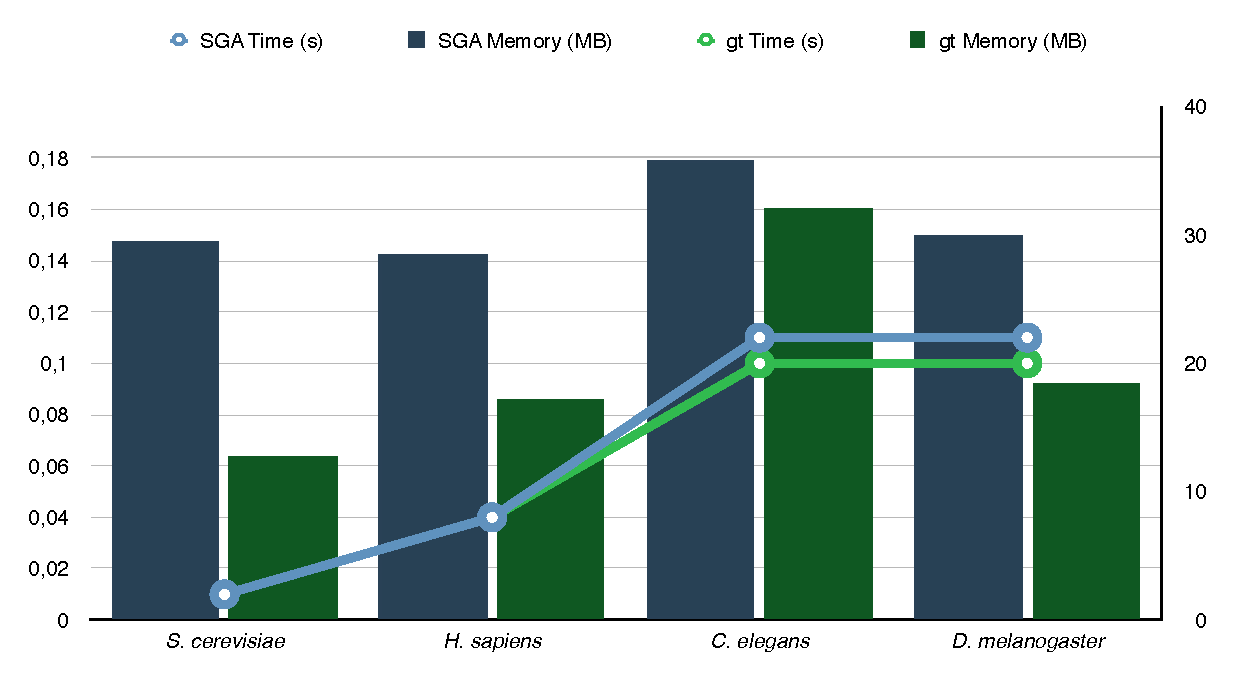
\includegraphics[width=\textwidth,height=0.8\textheight,keepaspectratio]{presentation/figures/sga_vs_gt.pdf}
  \caption{\label{abb: Zeit}Auftragung der Laufzeit und des
    Speicherplatzbedarfs von gt Scaffolder und SGA Scaffold für
    unterschiedliche Testdatensätze}
\end{figure}

In Abbildung \ref{abb: Zeit} sind die Laufzeiten und der
Speicherplatzbedarf der Programme gt Scaffolder und SGA Scaffold für
die verschiedenen Testdatensätze dargestellt. Die Testdatensätze sind
dabei der Größe nach von links nach rechts geordnet. Die Ergebnisse
von SGA Scaffold sind jeweils in rot dargestellt während die
Ergebnisse von gt Scaffolder grün eingefärbt sind.

Die Grafik verdeutlicht, dass gt Scaffolder sowohl bei der Laufzeit
als auch bei dem maximalen Speicherplatzbedarf entweder gleichauf mit
SGA Scaffold oder sogar besser ist.

Ebenfalls ist zu erkennen, dass die Laufzeit und der
Speicherplatzbedarf nicht mit der Größe der Referenzgenome
zusammenhängt. Allerdings hängen diese Punkte \todo{Punkte
  umformulieren?} auch nicht direkt von der Größe des Scaffoldgraphen
ab. In Tabelle \ref{tab: Vergleich} sind zu den Datensätzen die Anzahl
an Knoten in dem Scaffoldgraph dargestellt. So ist die Anzahl an
Knoten für den \textit{D. melanogaster} Datensatz mit $3970$ geringer
als für den \textit{H. sapiens} Chr. 21 Datensatz mit $4817$
Knoten. Trotzdem wird zur Berechnung der Scaffolds für den
\textit{D. melanogaster} Datensatz sowohl von SGA Scaffold als auch
von gt Scaffolder mehr Laufzeit und mehr Speicheplatz benötigt, wie
aus Tabelle \ref{tab: Vergleich} und Abbildung \ref{abb: Zeit}
ersichtlich wird. \todo{gehört dieser Abschnitt evtl in die Diskussion?}


\section{Diskussion und Ausblick}

\section*{Anhang}
\subsection*{Pseudocode}
(\todo{Algorithmen anpassen!!!})

\begin{algorithm}[H]
  \ForEach{Knoten $k_0$ im Graph $G$}{
    \ForEach{Kantenrichtung $dir$ in [ANTISENSE, SENSE]}{
      \ForEach{Kantenpaar $(A,B)$ in Richtung $dir$}{
        $k_1$ = $A.pend$\;
        $k_2$ = $B.pend$\;
        \If{AmbiguousOrdering($A,B,p\_cutoff$) {\bf and}
           $k_1.estCopy + k_2.estCopy < cn\_cutoff$}
          {
            \If{$k_1.estCopy < k_2.estCopy$}{
              markiere $k_1$ als polymorph und alle aus-
              und eingehenden SENSE und ANTISENSE Kanten von $k_1$
              schwarz, so dass sie im nächsten Schritt nicht
              mitbeachtet werden.\;
            }
            \Else {
              markiere $k_2$ als polymorph und alle aus-
              und eingehenden SENSE und ANTISENSE Kanten von $k_2$
              schwarz, so dass sie im nächsten Schritt nicht
              mitbeachtet werden.\;
            }
           \tcp{bei polymorphen Knoten wird nur das erste
             polymorphe Kantenpaar markiert}
           \If{Knoten $k_0$ ist polymorph markiert}{
             break\;
           }
          }
        }
      \tcp{polymorphe Knoten müssen nicht mehr auf
        inkonsistente Kanten überprüft werden}
       \If{Knoten $k_0$ ist polymorph}
         {break\;}
       \ForEach{Kantenpaar $(A,B)$ in Richtung $dir$}{
         \If{$A$ ist nicht schwarz und $B$ ist nicht schwarz}
            {
              Berechne Overlap von $A$ und $B$ und speichere
              längsten Overlap.\;
            }
       }
       \If{längster Overlap $>$ 400} {
	 Markiere alle ausgehenden Sense-/Antisensekanten
         von $k_0$ rot\;
      }
    }
  }
  Lösche alle markierten Knoten und Kanten\;
  \caption{\label{alg: Selektion}Zusammengefasste Filterfunktion (Schritt 4a und 4b vereinigt)}
\end{algorithm}

\begin{algorithm}[H]
  \KwData{Kante $A$ und Kante $B$, die auf eindeutige Ordnung geprüft werden
    sollen. Wahrscheinlichkeitsschwellenwert $p\_cutoff$}
  \KwResult{Ob die Kanten $A$ und $B$ nicht eindeutig geordnet werden können}
  $\mu = A.dist - B.dist$\;
  $\sigma^2 = A.\sigma^2 + B.\sigma^2$\;
  $t = \frac{-\mu}{\sigma\cdot\sqrt{2}}$\;
  $P_{AB} = \frac{1}{2} \cdot \left( 1 + \frac{2}{\sqrt{\pi}} \int_{0}^{t} \exp{-x^2}\mathrm dx\right)$\;
  $P_{BA} = 1 - P_{AB}$\;
  \Return $\max\{P_{AB}, P_{BA}\} \leq p\_cutoff$
  \caption{Funktion \textsc{AmbiguousOrdering}$(A, B, p\_cutoff)$}
\end{algorithm}


\begin{algorithm}[H]
  \KwData{Graph}
  \KwResult{Graph ohne Zyklen}
  \While{noch nicht fertig}{
  Suche alle Zusammenhangskomponenten\;
  \ForEach{Zusammenhangskomponente}{
    Suche alle terminalen Knoten\;
    \ForEach{terminalen Knoten}{
      Suche mit einer Tiefensuche nach Rückkanten zu diesem Knoten\;
      \If{Rückkante gefunden}{
        markiere den terminalen Knoten und den Knoten, von dem die 
        Rückkante ausgeht, als REPEAT\;
        }
      }
    }
  Lösche alle Knoten, die als REPEAT markiert sind\;
  }
  \caption{\label{alg: Zyklen}Löse Zyklen auf (Schritt 5)}
\end{algorithm}

\begin{algorithm}[H]
  \SetAlgoLined
  \KwData{Graph $G$}
  \KwResult{Graph $G$ ohne Knoten, die nicht zum bestem Walk gehören}
  Markiere alle Kanten aus $G$ schwarz\;
  Berechnung der Menge $C$ aller Connected Components von $G$\;
  \ForEach{Connected Component $c_0$ aus der Menge $C$}{
    Berechne Menge der terminalen Knoten $T$ (mit ausschließlich SENSE
    oder ANTISENSE Kanten) für die Connected Component $c_0$\;
    \ForEach{Terminaler Knoten $t_0$ aus der Menge $T$}{
      Berechne die Menge $W$ aller Walks durch die Connected
      Component $c_0$ von $t_0$ aus\;
      \ForEach{Walk $w_0$ aus $W$}{
        \If{Contig-Gesamtlänge > bislang beste Contig-Gesamtlänge}{
          Setze aktuellen Walk $w_0$ als bestWalk\;
        }
      }
    }
  }
  Setze alle Kanten des bestWalk weiß\;
  Lösche alle schwarzen Kanten\;
  \caption{\label{alg: Scaffold}Berechnung der Scaffolds (Schritt 6)}
\end{algorithm}

\begin{algorithm}[H]
  \SetAlgoLined
  \KwData{terminaler Startknoten $t_0$}
  \KwResult{Alle von diesem Knoten möglichen Walks}
  Konstruktionsrichtung = Richtung der vom terminalen Knoten $t_0$ ausgehenden Kanten\;
  \ForEach{Kante $A$ vom Knoten $t_0$ ausgehend (in Konstruktionsrichtung)}{
    $k_0$ = $A.pend$\;
    Speichere Startkante $A$ und Distanz $A.dist$ in Map an Position
    $k_0$ (für spätere Traversierung)\;
    Schiebe Startkante $A$ und Distanz $A.dist$ in Queue\;
  }
  \While{BFS über Queue nicht beendet}{
    Poppe Kante $A$ und Distanz $A.dist$ aus der Queue\;
    $k_0$ = $A.pend$\;
    \ForEach{Kante $B$ in Konstruktionsrichtung von $k_0$ aus} {
      $k_1$ = $B.pend$\;
      \If{Distanz zu aktuell betrachtetem Knoten $k_1$ $<$
        bisher ermittelte Distanz zu $k_1$ {\bf OR} Knoten $k_1$
        noch unbetrachtet}{
        Speichere Kante $B$ und Distanz $B.dist$ in Map an Position $k_1$\;
        Schiebe Kante $B$ und Distanz $B.dist$ in Queue\;
      }
    }
    \If{$k_0$ hat keine Kanten in Konstruktionsrichtung}{
      Schiebe Knoten $k_0$ in terminalSet\;
    }
  }
  \ForEach{Knoten $k_0$ in terminalSet}{
    Erzeuge Walk mithilfe einer Traversierung über die Map
  }
  \caption{Berechnung der Walks (Schritt 6.1)}
\end{algorithm}

\bibliography{presentation/literatur}
\bibliographystyle{alpha}

\end{document}
